\chapter[Bacgkround Free Imaging]{Background-free imaging of gold nanorods
through detection of anti-Stokes emission}
\label{ch:Imaging}

\blfootnote{This chapter has been published in Biophysical Journal (XX) NN.}

\begin{abstract}
Metallic nanoparticles have opened the possibility of
imaging, tracking and manipulating biological samples without time limitations.
Their low photoluminescence quantum yield however, makes them hard to detect
under high background conditions. In this study we show that it is possible to
image gold nanorods by detecting their anti-Stokes emission under resonant
excitation. We show that even in a cell containing the fluorescent dye $\atto$,
the signal-to-background ratio of the anti-Stokes emission is higher than 10,
while it is impossible to image the particles with the Stokes emission. The main
advantage of this technique is that it does not require any major change in
existing fluorescence imaging setups, only the addition of an appropriate
short-pass filter in the detection path.
\end{abstract}

\section{Introduction}
High-resolution microscopy has become an indispensable tool for studying
biological samples both in vitro and in vivo\cite{Moerner2007}.
Fluorescent organic dyes are commonly employed to such ends because of their
reduced size and high quantum yield\cite{Lichtman2005}. Fluorophores, however,
have an inherent constraint  in the possible observation time, since molecules
eventually bleach under intense illumination\cite{Shaner2005}. Even the most photostable
dyes cannot be imaged at saturation for longer than few tens of seconds. Gold
nanoparticles on the other hand are almost indefinitely stable\cite{Jana2001}
and open up many original applications including photothermal
therapy\cite{Alkilany2012} and imaging\cite{VandenBroek2013}.

As gold nanoparticles do not blink nor
bleach\cite{PEREZJUSTE2005,Mohamed2000},they are ideal candidates for
labelling\cite{Yao2014}, tracking\cite{Spillane2014} and
manipulating\cite{Urban2011} biological samples over extended periods of time.
Moreover it has been shown that with the proper size and coating, they do not
interfere with cells' functioning\cite{Lewinski2008}, allowing not only
\textit{in vitro} but also \textit{in vivo} studies. Compared to organic dyes,
gold nanoparticles are much larger and their emission quantum yield is much
smaller, in the order of $10^{-6}$\cite{Yorulmaz2012}. This minute value is
compensated by an absorption cross section several orders of magnitude larger
than that of molecules\cite{Link1999}, therefore the brightness of gold
nanoparticles is comparable to that of fluorescent molecules under the same
illumination intensity.

Since the absorption cross section of the particles scales as their volume, detecting
smaller particles in presence of background requires a specific approach.
Several techniques have been proposed, including two-photon
excitation\cite{VandenBroek2013}, photothermal \mbox{heterodyne}
detection\cite{Berciaud2006} and interferometric detection\cite{Ignatovich2006}.
Each of these methods are useful but their operation requires dedicated setups
and a high level of expertise. A method that allows to image gold nanoparticles with
a high background rejection and that is readily implementable in current
confocal and wide-field microscopes would provide great benefits.

Gold nanoparticles exhibit a collective oscillation of conduction electrons
called surface plasmon resonance\cite{Bouhelier2005}. This resonance strongly
depends on the shape of the particles\cite{Dulkeith2004}\cite{Link2000a}.
Spheres with radius roughly between $5$ and $80\nm$ will have a resonance
between $520\nm$ and $560\nm$; more elongated particles such as nano-rods or
bipyramids\cite{Rao2015} exhibit red-shifted longitudinal resonances that reach
wavelengths of $800\nm$ or longer\cite{Ngoc2015}. It is important to note that
tuning the shape of the particles can be easily achieved by synthesis and that
relatively narrow size distributions can be obtained\cite{Nikoobakht2003}.

The plasmon is responsible for enhanced absorption and scattering cross
sections\cite{Ni2008} of particles for specific wavelengths but it is also
responsible for enhanced photoluminescence emission in the spectral region of
the plasmon resonance. Because of the absence of a gap in the excited states
spectrum of gold nanoparticles, their photoluminescence excitation spectra
overlaps their emission spectrum\cite{Yorulmaz2012}, a very different situation
from the Stokes-shifted emission of fluorescent molecules and semiconductor
nanocrystals. Upon excitation of gold nanoparticles at their plasmon resonance
maximum, most of the emission will be concentrated in a narrow spectral region
around the excitation. This implies that most of the luminescence will be
blocked by the filters that, in fluorescence detection experiments, prevent
direct excitation light from reaching the detectors.

It is also possible to excite the particles off-resonance with a shorter
wavelength laser (for instance through interband transitions with $532\,\nm$)
and the emission will be mostly concentrated around the longitudinal plasmon
resonance of nanorods at longer wavelengths. This is the closest situation to
the behavior of a fluorophore, in which the Stokes-shifted emission can be
easily detected by introducing a long-pass filter. The drawback, however, is
that the cross section of particles is much smaller at this wavelength and can
only be compensated by increasing the excitation power.

\begin{figure}[htp] \centering
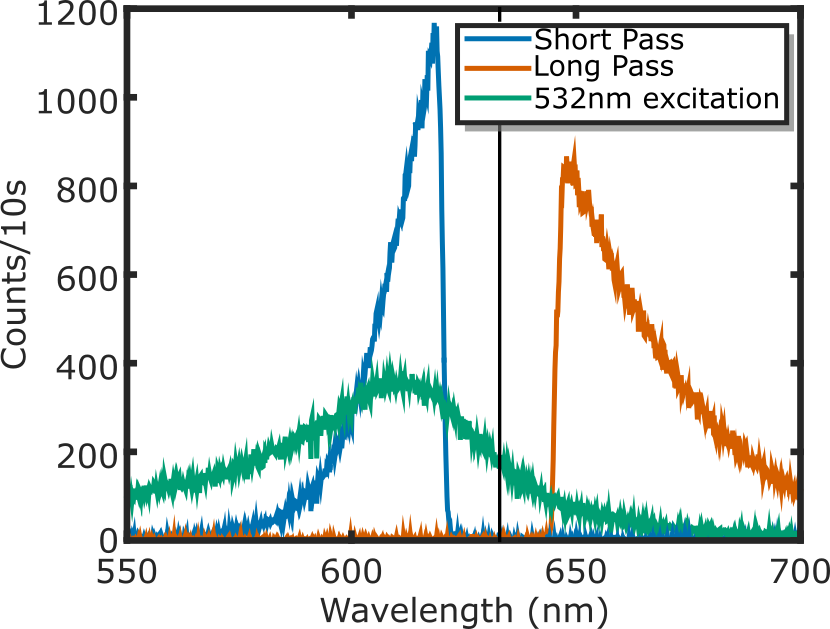
\includegraphics[width=0.45\textwidth]{Chapters/03_Background_Free/Figures/01_3_Curves/3_curves_final.png}
\caption{Luminescence spectra of a single gold nanorod. Green curve: emission
upon excitation with a $532\nm$ laser. Red curve: Stokes emission upon
excitation with a resonant $633\nm$ HeNe laser. Blue curve: anti-Stokes emission
under the same $633\nm$ excitation.}
	\label{fig:spectra_rod}
\end{figure}

Figure \ref{fig:spectra_rod} shows typical spectra of a gold nanorod under
different excitation wavelengths. The green curve is the one-photon-excited
luminescence spectrum around the longitudinal plasmon resonance, observed while
irradiating with $532\nm$ laser; the full spectrum of the longitudinal plasmon
is clearly observable with its resonance at $620\nm$. The particle can also be
excited at or close to its resonance, where its absorption cross section is
maximum. 

Figure \ref{fig:spectra_rod} shows the emission spectra upon excitation at
$633\nm$, depicted as the vertical black line. The red curve is the
Stokes-shifted emission; the spectral shape of this emission overlaps with the
one observed exciting at $532\nm$. Exciting in resonance is more efficient and
therefore the emission is much brighter. The blue curve in fig.
\ref{fig:spectra_rod} displays the anti-Stokes emission at shorter wavelengths.
In this case the spectral shape doesn't resemble that of the plasmon resonance.
The exponential-like decay of the anti-Stokes spectrum can be modelled with
Boltzmann statistics\cite{He2015} of the bath (phonons and electrons) energy
levels that are present in gold nanoparticles at room temperature. In both cases
it is clear from the shape of spectra that the filters block an important part of the
emission close to the plasmon maximum.
 
This work focuses in the exploitation of the anti-Stokes
luminescence\cite{Jiang2013} for imaging of gold nanorods in biologically
relevant conditions. This scheme benefits from the enhanced absorption cross
section of the particles, their high photo-stability and fairly narrow emission
spectra. When exciting in resonance with the plasmon, a short-pass filter can be
introduced allowing the observation of only the anti-Stokes emission. This
procedure is that it highly reduces the background arising from
self-fluorescence and Raman-scattering from cells, most of it being
Stokes-shifted. Reducing the background therefore opens the possibility of
imaging and tracking smaller particles or using lower excitation powers.

\begin{figure}[htp] \centering
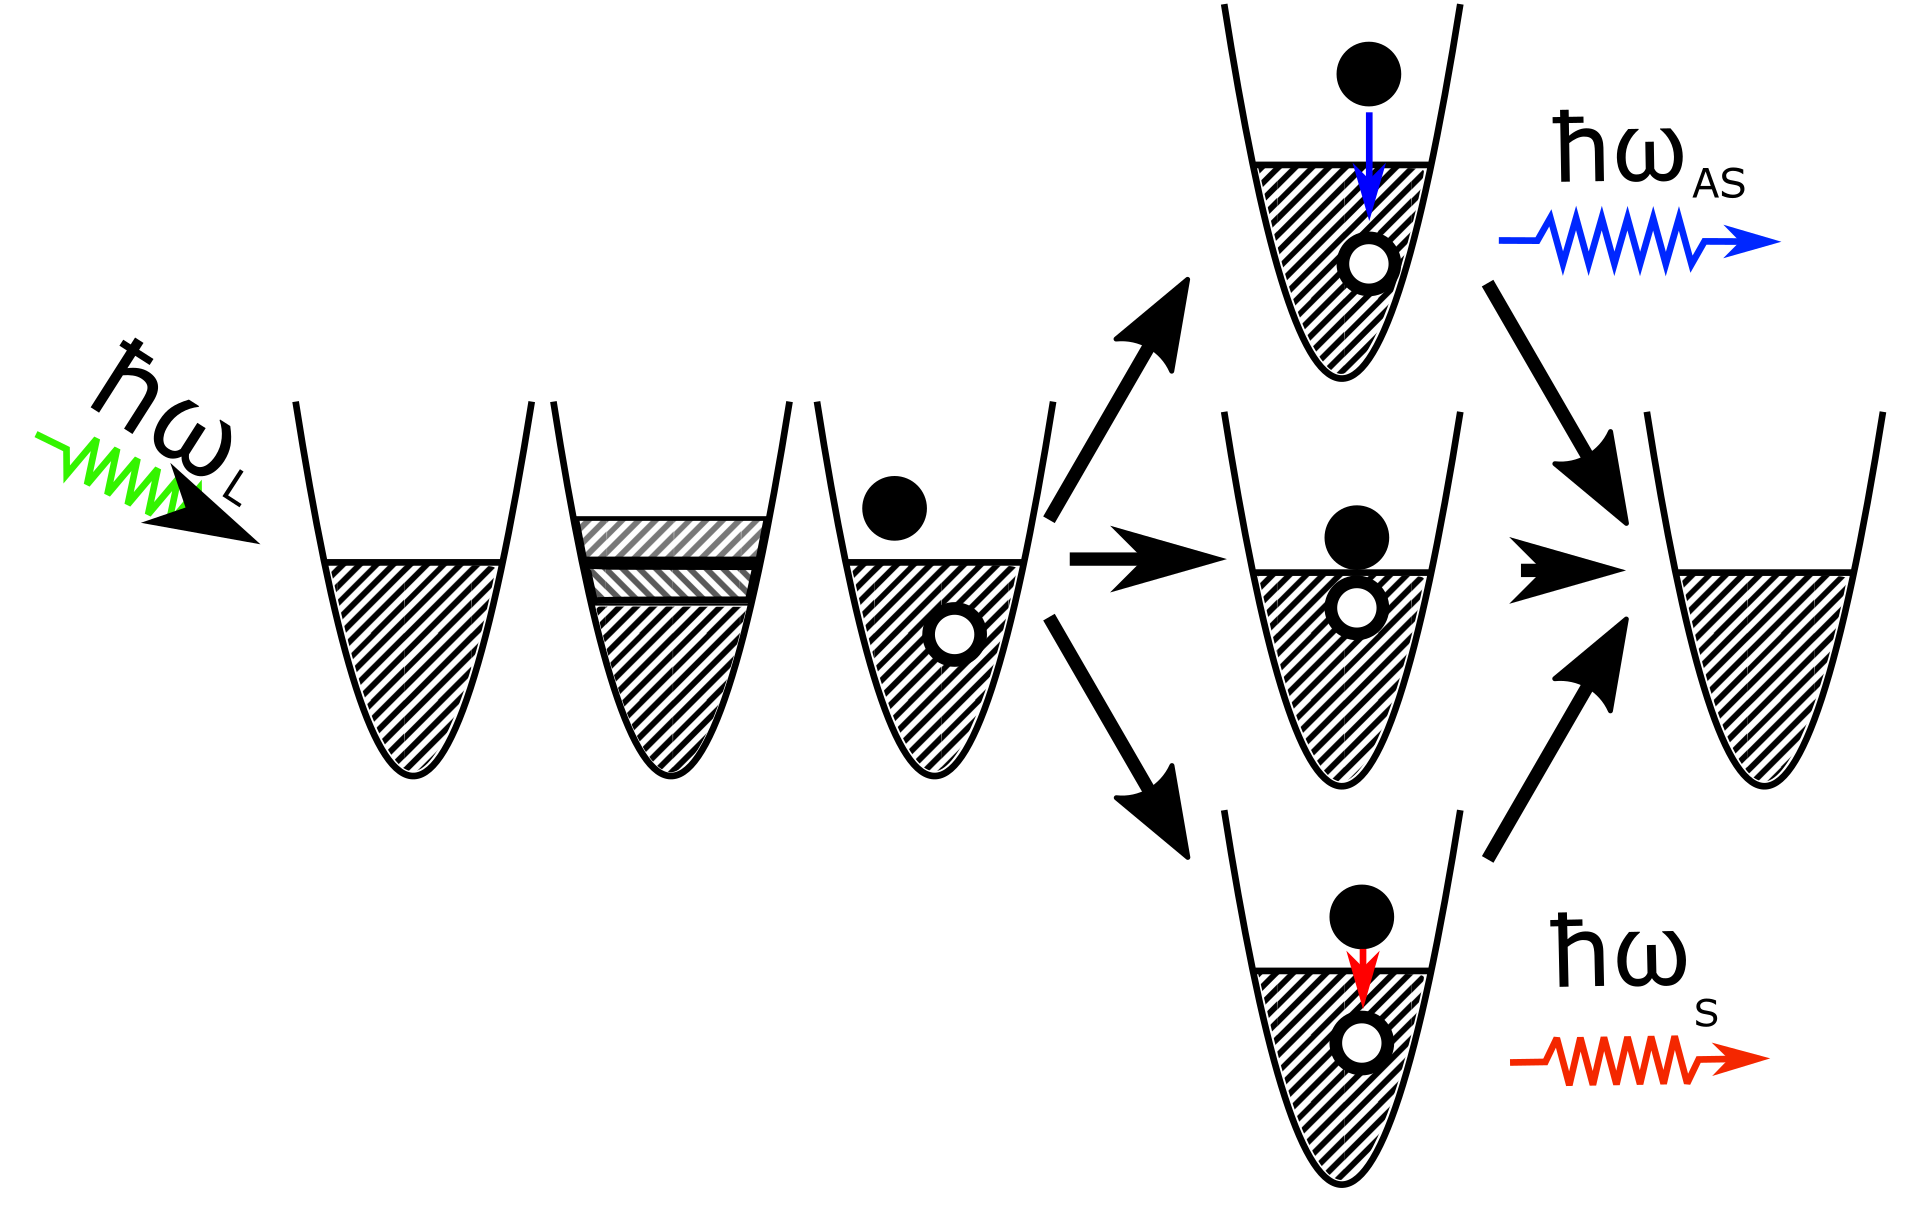
\includegraphics[width=0.45\textwidth]{Chapters/03_Background_Free/Figures/02_Scheme/luminescence_all_AS.png}
\caption{Schematic of the anti-Stokes luminescence arising from a single gold
nanorod. After excitation with a photon, a collective oscillation of electrons
is generated. Once the coherence is lost, the state can be described as an
electron-hole pair. Three scenarios are possible: electron and hole may
recombine radiatively after one of more interactions with the thermal baths of
lattice phonons and charge carrier thermal excitations: i) if the energy
difference between electron and hole states is lower than the initial one after
excitation we obtain Stokes emission upon a radiative recombination; ii) if
electron and hole transiently increase their energy difference at the bath's
expense before recombining radiatively, we observe anti-Stokes emission; iii) if
electron and hole recombine non radiatively, their energy difference is
transferred to the baths and no photon is emitted. The latter process is the
most probable one).}
	\label{fig:anti-Stokes-process}
\end{figure}

The anti-Stokes emission mechanism\cite{He2015} is depicted in Figure
\ref{fig:anti-Stokes-process} and can be described as follows: an absorbed
photon generates a collective oscillation of the conduction electrons. After a
fast loss of the coherence\cite{Sonnichsen2002}, the state of the particle can
be described as an electron-hole pair. After one or more interactions with the thermal
baths, i.e. with phonons of the gold lattice\cite{Lin2008} or thermally
excited charge carriers\cite{Sun1994}, the hole and/or the electron can
receive energy. This energy can transiently increase the energy difference between electron and
hole; if then they recombine radiatively, the emitted photon will have a shorter
wavelength (higher energy) than the incoming photon\cite{Huang2014}. The same
mechanism accounts for the Stokes-shifted emission, the only difference being
that the electron-hole pair has lost energy to the baths before recombining
radiatively. Finally, electron and hole can recombine
non-radiatively, transferring their whole energy to the lattice. 

\begin{sloppypar}
The probability of a radiative recombination of electrons and holes is low,
as can be experimentally determined by the very low emission quantum yield of
the photoluminescence\cite{Yorulmaz2012}\cite{Rao2015}\cite{Sonnichsen2002}. Anti-Stokes
emission stems from electron-hole recombination events after the electron-hole
pair has transiently gained energy from the lattice, i.e., before it thermalizes. Even if the
anti-Stokes scenario is unlikely, it is frequent enough as to observe an
intensity in the range of $10^3$ counts per second on an avalanche photodiode
with excitation powers around $16\pwr$. Such relatively high detection rates
require enhancement of the emission probability through the proximity of the
plasmon resonance\cite{Neupane2013}.
\end{sloppypar}

The main advantage of the approach presented in this work is the simplicity of
its implementation. With any confocal or wide-field setup enabling resonant
excitation of gold nano-particles, one can exploit the anti-Stokes
photoluminescence by inserting a proper short-pass filter in the detection path.
As we will see below, single gold nanoparticles can be detected even in higher background conditions
such as a stained cell, or a highly self-fluorescent sample.

\section{Experimental method}
Images of gold nanorods were recorded by sample scanning employing a XYZ piezo
stage (PI Nano Cube) in a  home-built confocal microscope, sketched in Figure
\ref{fig:setup}a. The objective employed was an oil-immersion Olympus 60X NA
$1.4$ that allowed a high efficiency in both exciting the particles and
collecting their emission. The luminescence arising from the particles was
filtered and detected by either an avalanche photodiode or a
liquid-nitrogen-cooled CCD-spectrometer (Acton $500\textrm{i}$). An example of
an image can be seen in Figure \ref{fig:setup}b. To detect the anti-Stokes
luminescence, a $633\nm$ short-pass filter (Semrock) was added to the detection
path together with a $633\nm$ notch filter. Both filters were needed
simultaneously since neither of them was able to entirely block the excitation
light from the detectors. The Stokes luminescence was collected replacing the
short-pass filter with a $633\nm$ long-pass (Semrock).

Gold nanorods were synthesized by following the standard seeded-growth
method\cite{Nikoobakht2003}. The average size of the nanorods was $50\nm\times
23\nm$ and their SPR was located at around $630\nm$ in water. Figure
\ref{fig:uvvis} shows the extinction spectrum of a suspension of the
nanoparticles after synthesis and Fig. \ref{fig:TEM} shows a TEM image of the
rods.

Two different laser wavelengths were employed. A $532\nm$ laser (CNI) was used
to excite the transverse plasmon and the full longitudinal plasmon
spectrum was collected. Single nanorods exhibit a narrow Lorentzian-shaped luminescence
spectrum as displayed in Figure \ref{fig:setup}c. A second laser (Thorlabs HeNe)
with a wavelength of $633\nm$ allowed us to excite the particles in resonance
and collect either the Stokes or the anti-Stokes emission depending on the
analysis filters.

\begin{figure}[htp] \centering
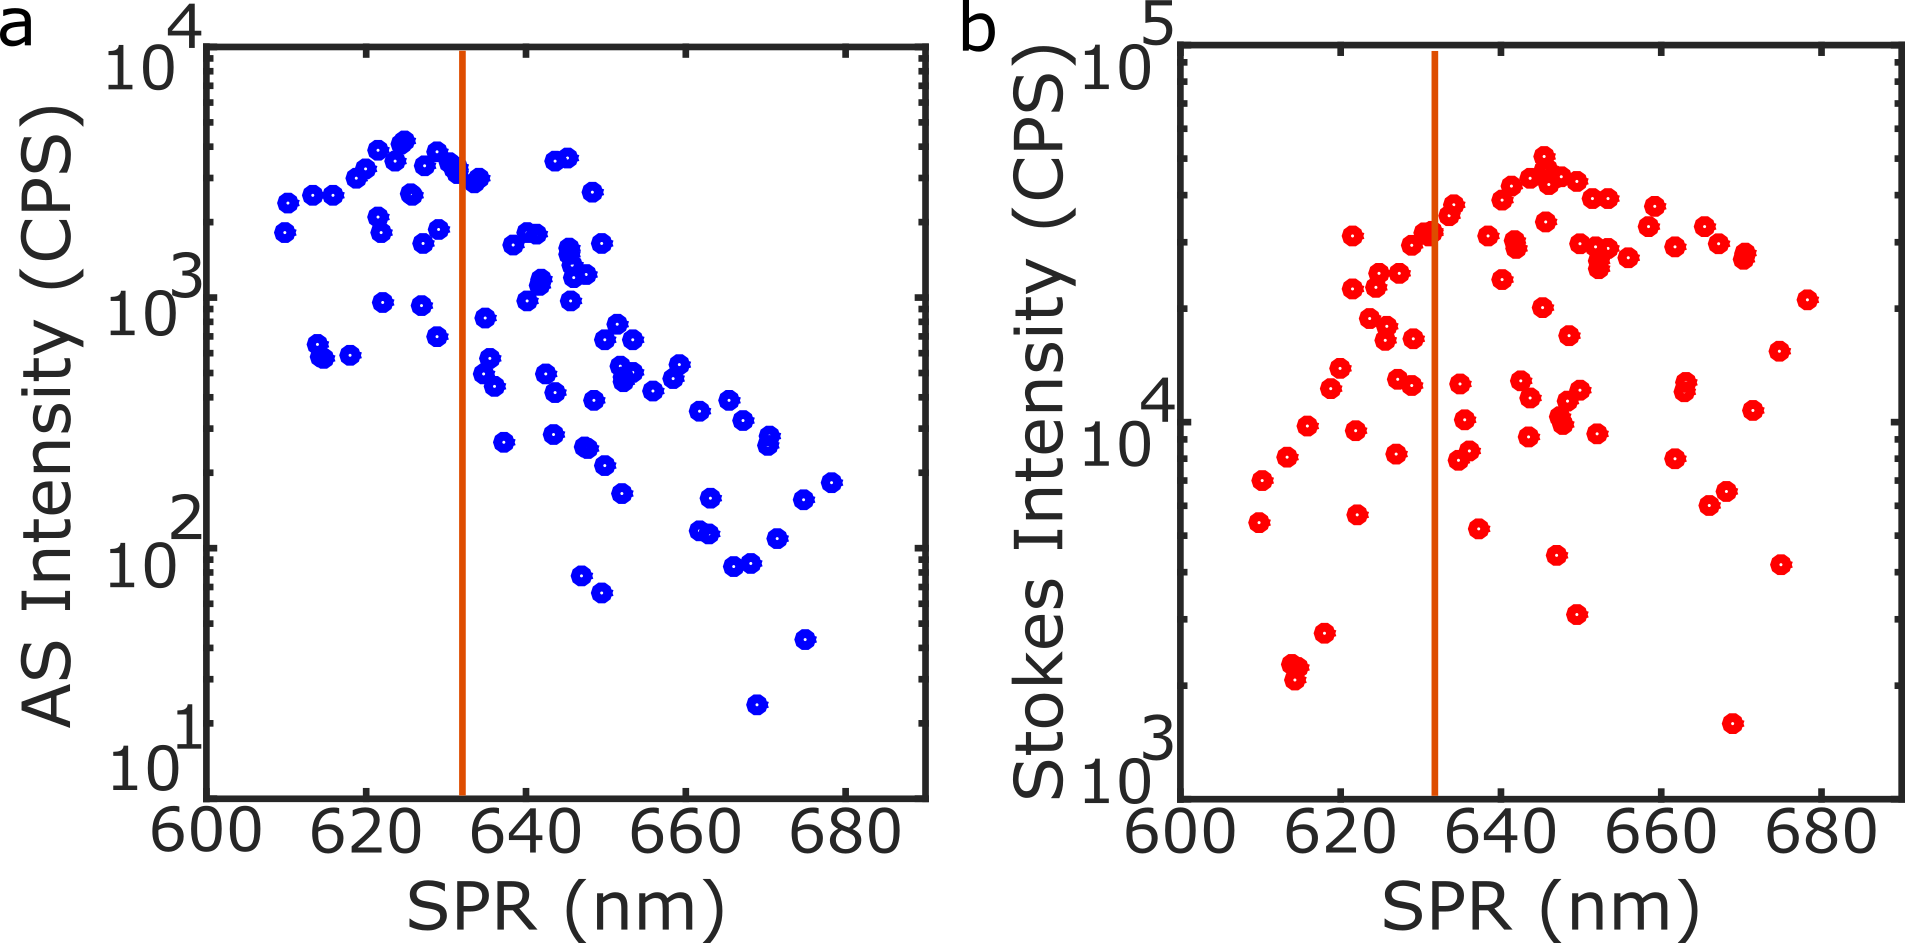
\includegraphics[width=0.45\textwidth]{Chapters/03_Background_Free/Figures/03_Intensity_SPR/Intensity_SPR.png}
\caption{Emission intensity of different gold nanorods as a function of their
plasmon peak position. The data are plotted for the anti-Stokes (a) and Stokes
(b) sides of the emission; the orange vertical line at $633\nm$ is the
wavelength of the laser. The spread in intensities for similar peak positions
can be attributed to variations in sizes and, possibly, to different quantum
yields of the different individual particles. The maximum emission for the
anti-Stokes is obtained when the plasmon is slightly blue shifted from the
excitation laser and viceversa for the Stokes emission.}
	\label{fig:emission_peak_position}
\end{figure} 

Figure \ref{fig:emission_peak_position} shows a scatter plot of the Stokes and
anti-Stokes emission intensities of $75$ gold nanorods against their plasmon
peak position. The large dispersion of the points observed can be attributed to
the distribution of sizes of the rods inherent to the synthesis
method\cite{Zijlstra2011} (bigger particles will have a bigger cross section)
and probably to different photoluminescence quantum yields for different
individual particles. Because the particles were first deposited on glass
directly and because they were excited with circularly polarized light, their
orientation shouldn't influence their photoluminescence intensity. It is
possible to observe that the maximum emission intensity for the anti-Stokes
appears for those particles with their plasmon slightly blue-shifted from the
laser wavelength, while the opposite is observed for the Stokes emission. This
means that there is a trade-off between the excitation efficiency and the
collection efficiency: exciting in perfect resonance is more efficient, but the
filters will eliminate most of the luminescence. Therefore exciting slightly to
the blue (red) of the resonance will be beneficial for the (anti-)Stokes
imaging.

To prove that the technique is well suited for imaging particles in
biological systems, we deposited HeLa cells on top of the nanorod sample.
Firstly, nanoparticles were deposited on clean glass coverslips by spin casting
a suspension of gold nanorods as described elsewhere\cite{Zijlstra2011}. This
procedure ensures that the analysis is performed on single nanorods and
therefore that the luminescence signals are not arising from clusters of
nanorods. It also allowed us to characterize the nanorod emission both by
acquiring spectra and by studying the dependency with excitation power, avoiding
the diffusion away from the focus.

Secondly, HeLa cells were plated on top of these samples, and grown overnight
until they reached a high confluency. Although the obtained images are not
equivalent to images of gold nanorods residing in the cytoplasm or nucleus of
cells, they would resemble very closely images of rods in cell membranes. This
simplified protocol only serves the present purpose of optical
signal-to-background characterization, and spared us the labour-intensive
bio-compatible particle functionalization that would be needed for more relevant
biological assays. Figure \ref{fig:white-light} shows a typical white light
transmission image of the samples. The high confluency ensures that cells
uniformly cover the entire observed area, so the studied nanorods are always
localized below a cell. We have also acquired images of nanoparticles under
cells containing the fluorescent dye $\atto$. For this purpose the cells already
attached to the coverslips were incubated with $45\pM$ $\atto$ for approximately
twenty minutes. This set of experiments allowed us to compare Stokes and
anti-Stokes emissions under high-background conditions.

\section{Results and discussion}

The nanoparticle shown in Fig. \ref{fig:spectra_rod} displays comparable count
rates for both the Stokes and anti-Stokes emissions. As explained earlier and
shown in Figure \ref{fig:emission_peak_position}, this is because the excitation
laser is slightly red-shifted from the plasmon resonance, the most favorable
position for enhancing the anti-Stokes part of the spectrum. Both types of
emission are also comparable to the luminescence intensity obtained while
exciting at $532\,\nm$. The main difference is the laser intensity employed; the
power density for exciting the transverse plasmon with the $532\nm$ laser was
set to $80\pwr$, while for both the anti-Stokes and Stokes, the $633\nm$ laser
was set to $15\pwr$, $5$ times less intense. This suggests that the enhancement
of absorption cross section at resonance more than compensates the loss of a
significant fraction of the luminescence emission in the laser rejection filter,
allowing us to use lower powers.

The three curves in Figure \ref{fig:spectra_rod} also show a very distinctive
spectral distribution. The luminescence that arises from the $532\nm$ excitation
spans almost $150\nm$, from the laser wavelength up to more than $650\nm$. The
Lorentzian shape confirms that the emission arises from a single nanorod. The
long-pass emission (red curve) spans a range of almost $100\nm$, from the
excitation at $633\nm$ to above $700\nm$. Finally, the anti-Stokes emission,
which requires energy extraction from the thermal bath cannot extend much beyond
a few $\textrm{k}_{B}\textrm{T}$ from the excitation energy. This is the
narrowest band, extending from the excitation to about $580\nm$. The position of
the plasmon resonance to the blue of the excitation laser explains the higher
peak intensity of the anti-Stokes spectrum compared to the Stokes spectrum,
whereas the total integrated Stokes emission is higher than the anti-Stokes's.

\begin{figure}[htp] \centering
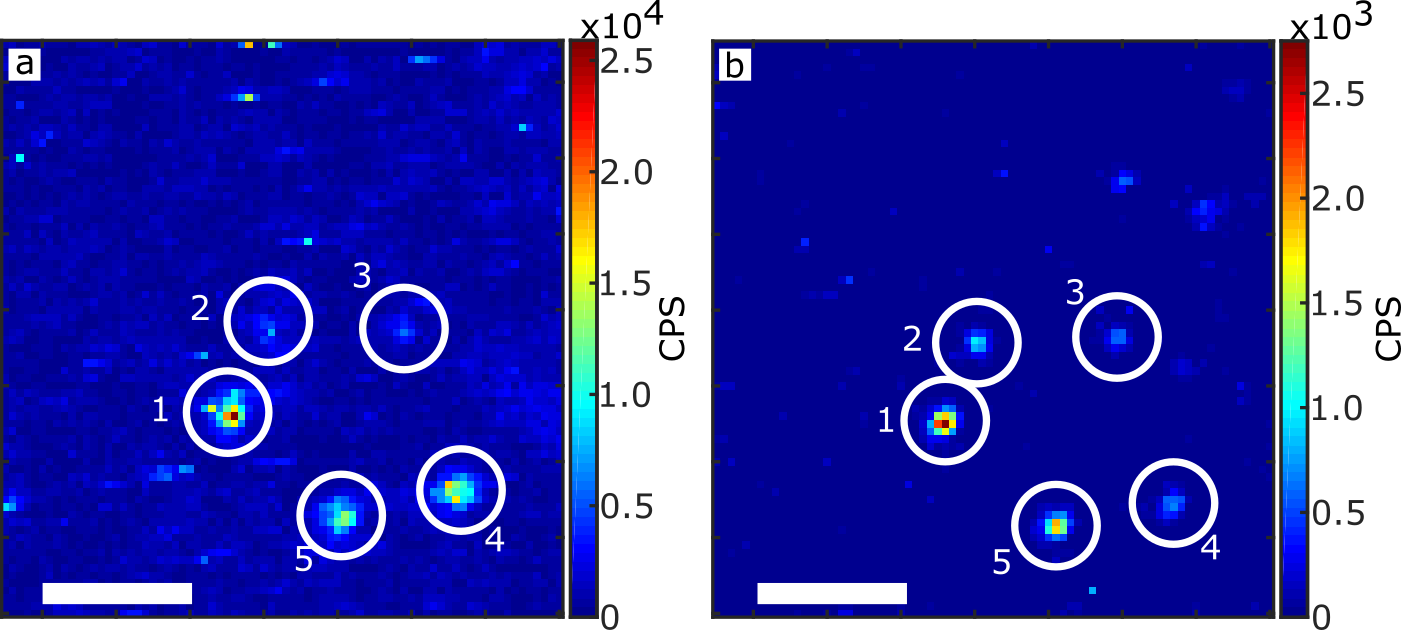
\includegraphics[width=0.9\textwidth]{Chapters/03_Background_Free/Figures/04_Stokes_AS/stokes_as_no_dye.png}
\caption{Raster scan of a nanorod sample under HeLa cells using (a) a long pass
filter and (b) a short pass filter for photoluminescence detection.
Some rods can be observed in both images, some others only in the Stokes or
anti-Stokes images. Intensities in the Stokes and anti-Stokes emission thus do
not necessarily correlate. The scale bar in both figures is $2\um$ in length.}
	\label{fig:stokes_as_no_dye}
\end{figure}

Figure \ref{fig:stokes_as_no_dye} shows two raster scans of the same
$7.5\times7.5\um^2$ area of the sample with HeLa cells on top of gold nanorods.
The left image shows the Stokes emission, where a $633\nm$ notch and $633\nm$
long pass filter were employed. The right image corresponds to the anti-Stokes
emission, where the same notch and a $633\nm$ short pass filter were employed.
In both cases the irradiation intensity was kept at $30\pwr$ at the back
aperture of the objective. Most particles are observed in both Stokes and anti-Stokes images
but with different intensities. The main difference between the two images is
the background count rate. The Stokes image has an average count rate around
$5\textrm{k}\CPS$, while the anti-Stokes is below $100\CPS$, close to the dark
counts of the detector. Moreover in the Stokes image a structured background can
be observed; we attribute this emission to self-fluorescence of the cells. On
the other hand, the anti-Stokes image shows a much flatter background and highly
distinguishable single particles. Both images display the count rate
obtained after dark count subtraction.

The circled particles in fig. \ref{fig:stokes_as_no_dye} show the different
possible situations: Particle $1$ is the brightest both in Stokes and
anti-Stokes and can be explained if this is a bigger particle.
Particles $2$ and $3$ are barely distinguishable in the Stokes image, while they
are clearly visible in the anti-Stokes. This can be attributed to a higher
background level in the Stokes case and by a plasmon resonance of particles $2$
and $3$ to the blue of the laser, favoring the anti-Stokes emission process.
Particles $4$ and $5$ are visible in both, but particle $4$ is brighter than $5$
in the Stokes image, while the opposite happens in the anti-Stokes.
This is due to a plasmon position that favors more one or the other type of
emission, as also shown in fig. \ref{fig:emission_peak_position}. Figure
\ref{fig:full_no_dye} shows a larger area of the scan, where it is possible to
observe more particles both in the Stokes and anti-Stokes configuration.

The use of the anti-Stokes emission is highly especially valuable when imaging
nanoparticles in high background conditions. To this end we incubated the cells
with a solution of $\atto$. The fluorescent labelling of the cell, even if not
specific, resulted in a similar situation to what would be obtained in the case
of labelling organelles or the entire cell membrane. This dye was chosen because
its absorption maximum is close to $633\nm$, the excitation wavelength we
employed in these experiments, but also because of its photostability and high
quantum yield.

\begin{figure}[htp] \centering
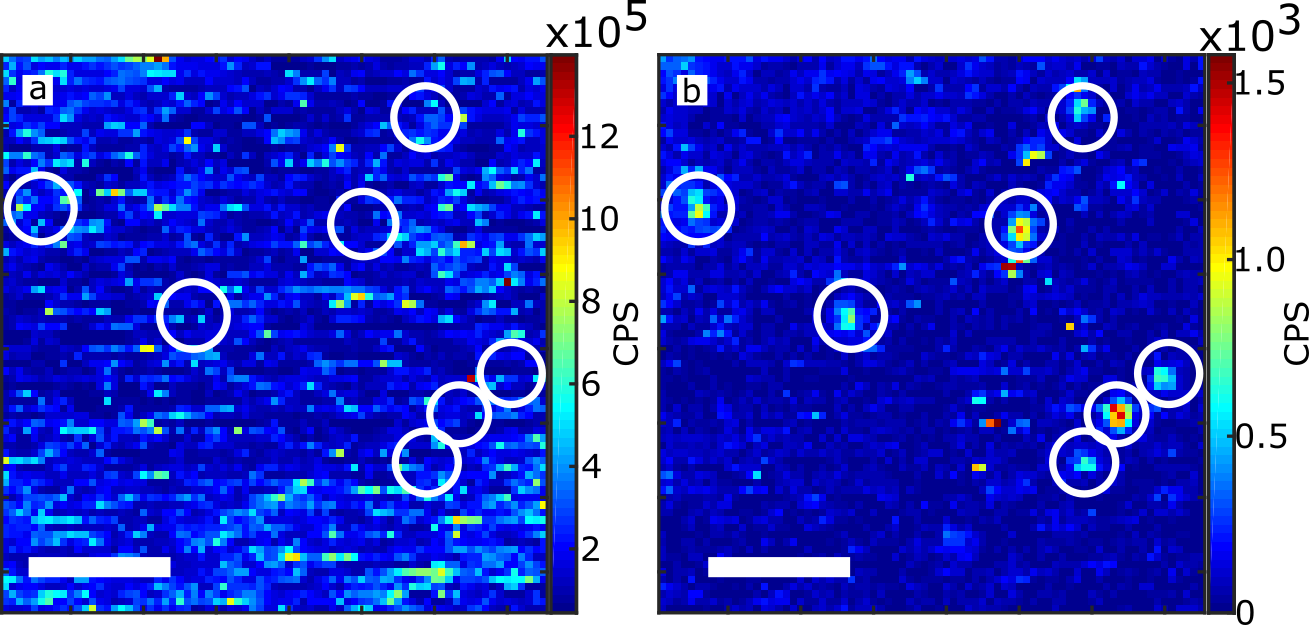
\includegraphics[width=0.9\textwidth]{Chapters/03_Background_Free/Figures/05_Stokes_AS_with_dye/stokes_as_with_dye.png}
\caption{Raster scan of a nanorod sample covered by HeLa cells containing the
fluorescent dye $\atto$, again using (a) a long pass filter and (b) a short pass
filter for photoluminescence detection. No clear nanorod signals can be seen in
the Stokes images, whereas they are clearly distinguishable in the anti-Stokes
image, proving the advantage of the latter for fluorescence background
rejection. The scale bar in both figures is $2\um$ in length.}
	\label{fig:Stokes_AS_with_dye}
\end{figure}

Figure \ref{fig:Stokes_AS_with_dye} shows two raster scans of the samples
described above. The right panel shows the anti-Stokes image, in which single
particles are clearly distinguishable and marked with a circle. We made sure
that the observed spots were nanorods by monitoring their intensity under high
illumination conditions and checking that they did not bleach. The left panel
shows the Stokes emission, in which no particles can be distinguished from the
background. The average emission in the anti-Stokes image is below $500\CPS$,
but higher than the dark counts of the detector. The Stokes emission, on the
other hand shows an average intensity around $200\kCPS$, one order of magnitude
higher than that observed without the dye.

These results indicate that the Stokes image deteriorates much faster than the
anti-Stokes in the presence of emitting molecules both from the cell itself or
from added dyes. The images show regions with higher emission intensities in
both configurations, most probably due to a higher concentration of dye in
specific regions of the cell. Figure \ref{fig:full_with_dye} shows a larger
scan, and the difference in background intensities is more evident. At much
higher concentrations than the ones shown in this work, the anti-Stokes emission
from the dye becomes significant and can overcome the emission rate from
individual particles.

\begin{figure}[htp] \centering
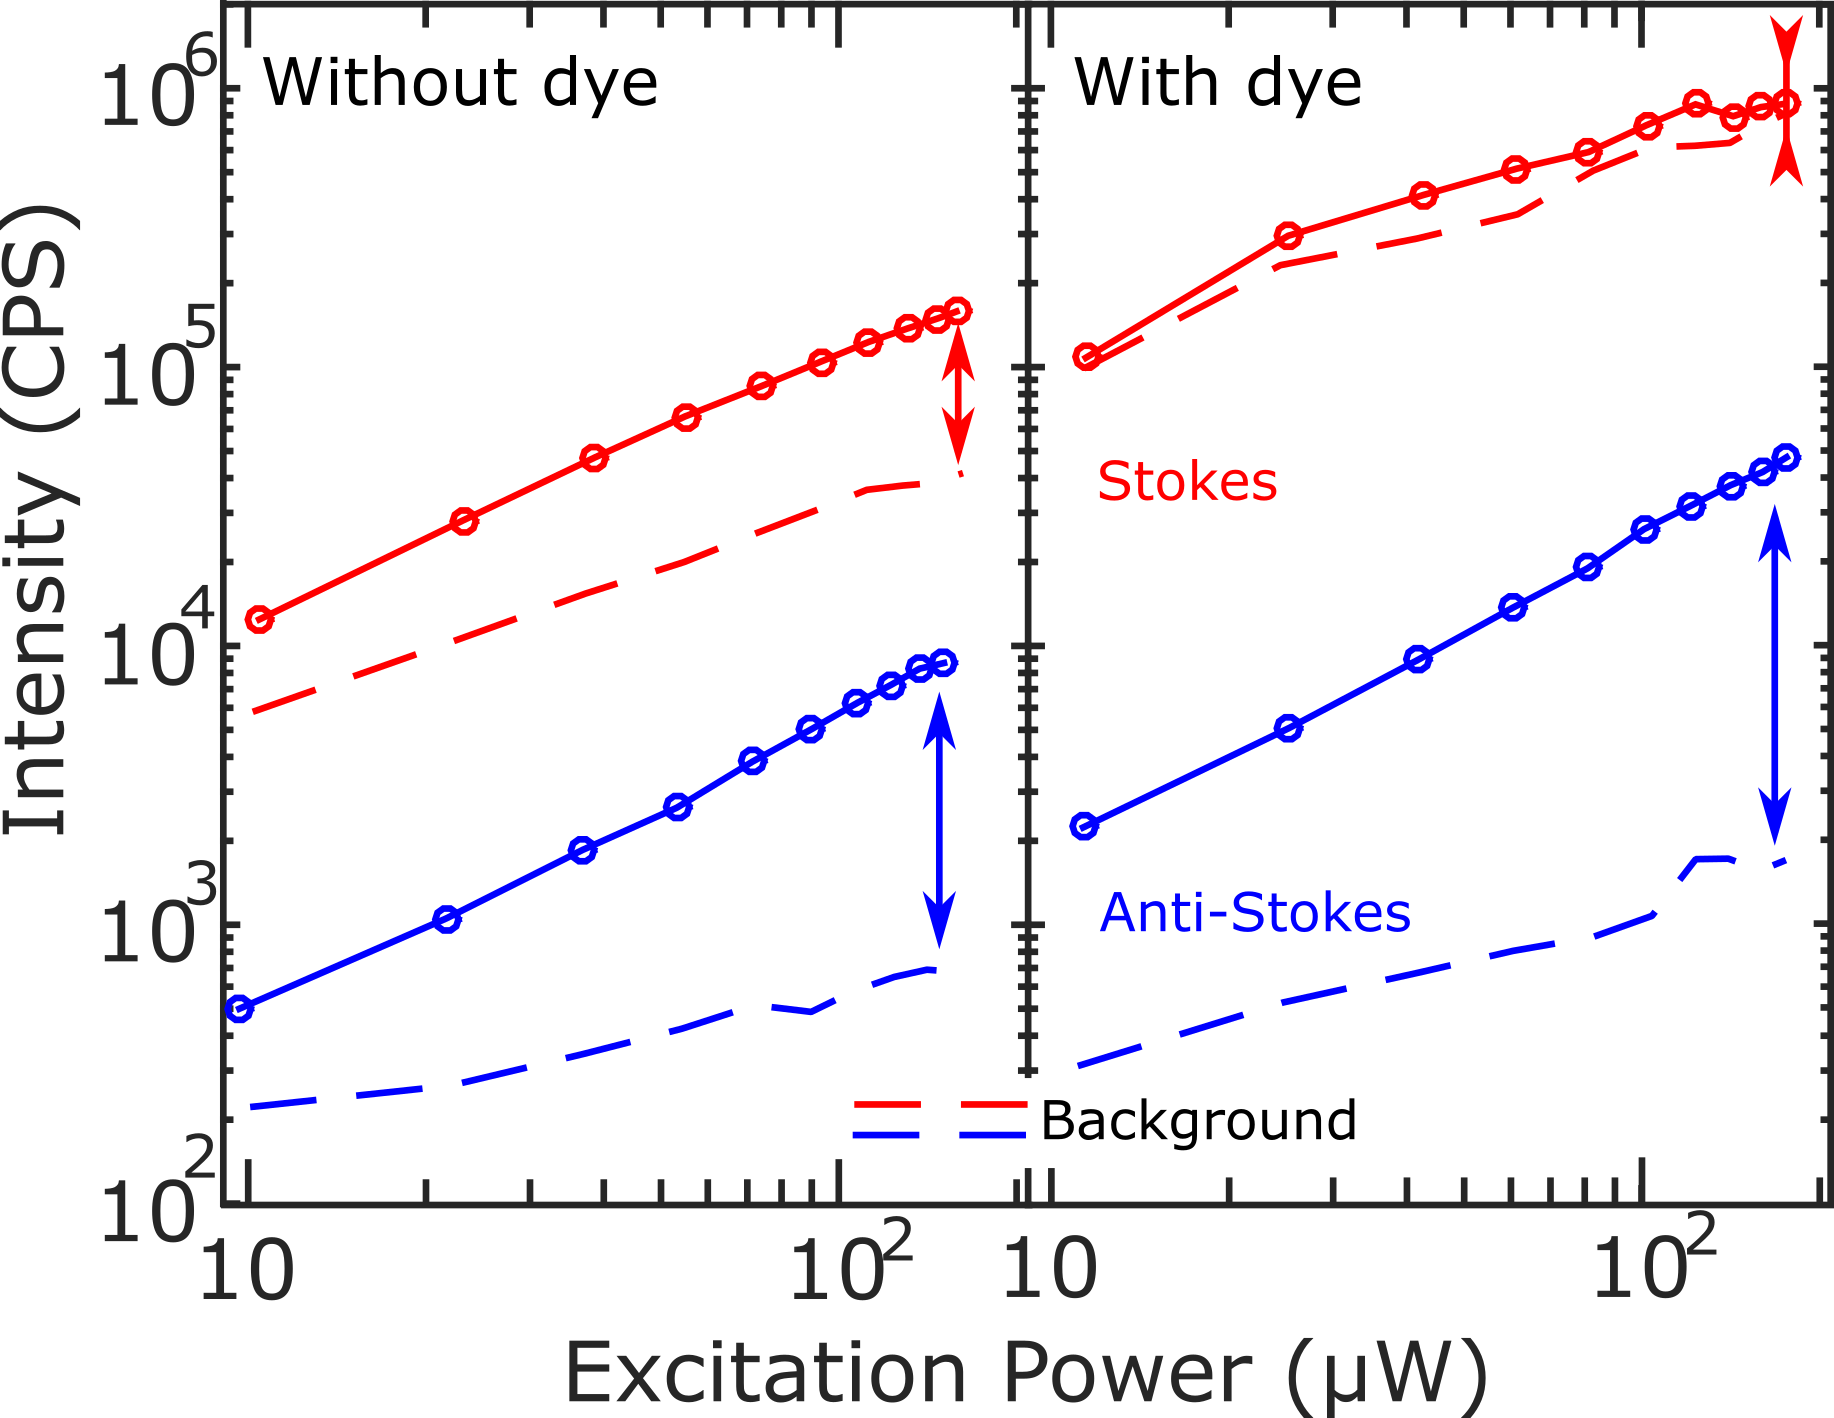
\includegraphics[width=0.45\textwidth]{Chapters/03_Background_Free/Figures/06_Power_Intensity/power_intensity.png}
\caption{Emission intensity (solid lines) and background (broken lines) as
functions of excitation intensity for the Stokes (red) and the anti-Stokes
(blue) emissions. These data were obtained on two different particles for the
right (unstained cells) and left (stained cells) panels. For the unstained
cells, the plasmon was chosen close to the laser line, so as to avoid favouring
one or the other emission by the resonance effect. Arrows indicate the maximal
signal-to-background ratio of each emission in the figure conditions. }
	\label{fig:power_intensity}
\end{figure}

Figure \ref{fig:power_intensity}a shows the dependence of the acquired
luminescence and the background as functions of excitation power for both the
Stokes and anti-Stokes emissions of a particle below a cell without dye. Care
was taken in choosing a particle with a resonance close to the excitation laser,
to compare Stokes and anti-Stokes luminescence with similar resonant
enhancements. The Stokes emission (red curves) shows a linear increase in signal
together with a linear increase in background. In this case the
signal-to-background ratio reaches a value of $6$. The anti-Stokes emission
(blue curves) however shows a much steeper increase of the signal than the
background, reaching a signal-to-background ratio of $12$. Of course, particles
with a plasmon resonance to the blue of the laser wavelength show an even larger
ratio of anti-Stokes to Stokes emission.

Figure \ref{fig:power_intensity}b shows the same type of curves as
\ref{fig:power_intensity}a, for a different particle under cells that contained
$\atto$. In this case the background prevented the acquisition of luminescence
spectra; the particle chosen to draw the figure is representative of the average
behavior. We see that in the Stokes case the particle's signal is barely larger
than the fluorescence background from the dye. On the other hand, the
anti-Stokes luminescence shows an enhanced contrast, reaching a
signal-to-background ratio of more than $20$ for this particular nanorod. The
background level observed in the Stokes image increases much faster with dye
content than the anti-Stokes background.

When the cells containing $\atto$ were used, we observed an increase in the
background levels for both Stokes and anti-Stokes emission and these levels also
depend on excitation power. This means that the dye shows both
components, as is well known from fluorescence hot bands and anti-Stokes Raman
scattering. The main difference between nanoparticles and dyes, however, is
their quantum yield. While the particles appear to be relatively bright
anti-Stokes emitters, in part due to their large absorption cross section, in
part due to their plasmon resonance, dyes such as the one employed in this work,
are much better Stokes emitters than anti-Stokes. This is the main reason why
rods are drowned by the fluorescence background in the Stokes image.

The signal-to-background ratio of the anti-Stokes emission increases with
increasing laser excitation powers, going from values close to $2$ for $3\pwr$
excitation up to values of $20$ for $53\pwr$ as shown in fig
\ref{fig:power_intensity}b. However this can't be extrapolated further than the
results presented here. It is known that gold nanorods reshape under high
irradiation intensities\cite{Liu2009}. For high-NA objectives like the one
employed in this work, a rule of thumb to prevent reshaping in scanning confocal images is to
keep the excitation intensity lower than $150\uW$ at the back aperture of the
objective lens (or equivalently a power density of $53\pwr$ at the object
plane.)

In the presence of a fluorescent dye, the signal-to-background obtained is
higher than in the case without dye. This may be a consequence of the selection
of particles with a plasmon more favorable to the anti-Stokes than to the Stokes
emission, and couldn't be avoided by acquiring luminescence spectra since the
background was too high. Although we checked the correct focusing on the sample
plane both by optimizing the reflection on the glass/water interface and by
employing the anti-Stokes signal, it was never possible to observe single
particles under high background conditions in the Stokes configuration.

\section{Conclusions}
In this work we have demonstrated that anti-Stokes photoluminescence arising
from the excitation in (or close to) the plasmon resonance of a gold nanorod can be
exploited to image them in biologically relevant conditions\cite{Jiang2013}. The
comparison between the Stokes and anti-Stokes emissions was possible by using
particles immobilized on the substrate, but this work shows that the technique
can be easily extended to imaging in fixed cells, \textit{in vivo} or even for
tracking particles in real time\cite{VandenBroek2013}.

Extending this technique to wide-field should be possible considering the laser
powers employed in this work. EMCCDs provide enough gain\cite{Dussault2004} to
easily detect single nanoparticles, while at the same time the background is
sufficiently low to give a high contrast. This extension of the technique would
open the possibility to track at higher frame rates than achievable by
confocal imaging.

The lower count rate of the anti-Stokes compared to the Stokes emission can be a
drawback in such applications as localization\cite{Sahl2013}. This technique's
accuracy depends on the number of photons detected, and is given by $\approx
1/\sqrt{N}$, where $N$ is the number of photons collected. The count rates
obtained in this work are close to $1.5\kCPS$, enough in many applications.

We have shown that the signal-to-background ratio of the anti-Stokes emission is
higher than that of the Stokes emission. In the case of HeLa cells not containing a
fluorescent dye, typical values can be around $10$ and $5$ respectively for a
particle with a resonance at the laser wavelength. For HeLa cells containing
$\atto$ the difference is much more pronounced, since most of the particles will
have a Stokes emission comparable or lower than the background, while in the anti-Stokes the
signal-to-background ratio can still be higher than $10$.

The main advantage of the technique presented in this work is that it can be
easily implemented in any commercial or home-built microscope. It does not
require a high investment in equipment or time, since filters are normally
available for common laser wavelengths and there is no further need of modifying
any experimental configuration already existent. Moreover all the data analysis
techniques employed in confocal or wide-field images for localization, tracking,
etc. do not have to be modified.

\section{Author Contributions}
AC performed the experiments, analyzed data and wrote the article. VIPK
prepared the samples and performed the experiments. MJMS designed the study. MO
designed the study and wrote the article. All authors analyzed the results and
approved the final version of the manuscript.

\section{Acknowledgements}
We thank Aimee Boyle for the synthesis and TEM images of the gold nanorods.
This work is part of the research programme of the Foundation for Fundamental
Research on Matter (FOM), which is part of the Netherlands Organisation for
Scientific Research (NWO).

\references{Chapters/03_Background_Free/BackgroundFree}